Magnetinės indukcijos linijos sukurtos tiesiu laidininku tekančios
srovės sudaro koncentrinių apskritimų, supančių laidininką sistemą.

\begin{exmp}
  Suraskime magnetinio lauko indukciją plono apskritimo pavidalo
  laidininko (spindulio ilgis – $R$) centre ir ašyje.

  TODO: Išsiaiškinti.

  Kiekvienas srovės elementas sukuria indukciją $d\vec{B}$, nukreiptą
  teigiama normalės kryptimi. Taigi gauname, kad magnetinė indukcija
  centre:
  \begin{align*}
    d B
    &= \frac{\mu_{0}}{4\pi} \frac{I dl}{R^{2}} \sin \alpha \\
    \intertext{kadangi $\alpha = \frac{\pi}{2}$, tai}
    &= \frac{\mu_{0}}{4\pi} \frac{I dl}{R^{2}} \\
  \end{align*}
  Integruojame pagal visą kontūrą:
  \begin{align*}
    B
    &= \frac{\mu_{0}I}{4 \pi R^{2}} \oint dl \\
    &= \frac{\mu_{0}I}{4 \pi R^{2}} 2 \pi R \\
    &= \frac{\mu_{0}}{4 \pi} \frac{2 \left( I \pi R^{2} \right)}{R^{3}} \\
    &= \frac{\mu_{0}}{4 \pi} \frac{2 p_{m}}{R^{3}} \\
  \end{align*}
  čia:
  \begin{description}
    \item[$p_{m}$] – apskritiminės srovės dipolinis magnetinis momentas,
      $p_{m} = I \pi R^{2} = IS$ ($\vec{p_{m}} = I S \vec{n}$).
  \end{description}

  Magnetinė indukcija ašyje (TODO: Pridėti brėžinį iš dėstytojo konspekto):
  \begin{align*}
    d B_{||}
    &= d B \sin \beta \\
    &= d B \frac{R}{b} \\
    &= \frac{\mu I R}{4 \pi b^{3}} dl \\
  \end{align*}
  Mums rūpi tik $d B_{||}$, nes kita sudedamoji dėl simetrijos yra
  lygi 0. Suintegravę pagal visą kontūrą gauname:
  \begin{align*}
    B
    &= \int d B_{||} \\
    &= \frac{\mu_{0} I R}{4 \pi b^{3}} \oint dl \\
    &= \frac{\mu_{0} I R}{4 \pi b^{3}} 2 \pi R \\
    &= \frac{\mu_{0}}{4 \pi} \frac{2 I \pi R^{3}}{4 \pi b^{3}} \\
    &= \frac{\mu_{0}}{4\pi}
      \frac{2 p_{m}}{\left( R^{2} + r^{2} \right)^{\frac{3}{2}}}
  \end{align*}
\end{exmp}

Iš \ref{eq:bsl_sin} nesunku gauti ir taškinio judančio krūvio
sukuriamą magnetinę indukciją, prisiminus formulę
$I = j \cdot S = e n v S$:

TODO: Išsiaiškinti ir suprasti. (Fizika12.png)

Magnetinis momentas:
\begin{equation*}
  \vec{p_{m}} = IS
\end{equation*}

\begin{figure}[H]
  \begin{center}
    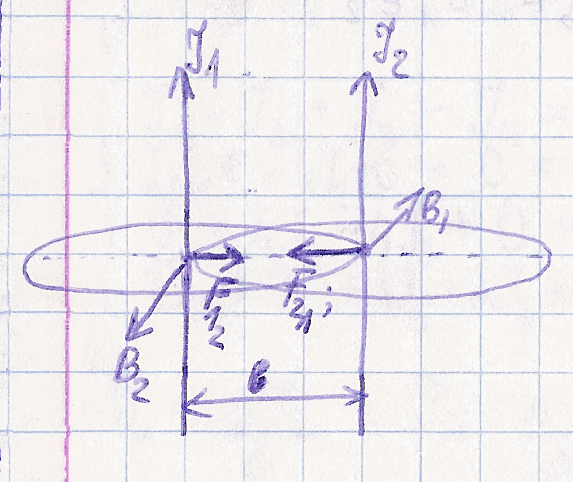
\includegraphics[height=0.5\textwidth]{images/bio_savaro_laplaso.png}
  \end{center}
  \caption{Bio-Savaro-Laplaso}
  \label{fig:bio_savaro_laplaso}
\end{figure}

\begin{defn}[Bio-Savaro-Laplaso dėsnis]
  Tarkime, kad turime du lygiagrečius begalinius laidininkus (žr.
  \ref{fig:bio_savaro_laplaso}), kuriais teka atitinkamai $I_{1}$
  ir $I_{2}$ stiprumo srovė, o tarp jų yra $b$ metrų tarpas.
  \begin{align*}
    \intertext{Tada pirmojo laidininko, antrojo laidininko taške,
    sukuriama indukcija bus lygi:}
    B_{1} &= \frac{\mu_{0}\mu 2 I_{1}}{4 \pi b} \\
    \intertext{Antrojo laidininko $dl$ ilgio atkarpą veiks jėga:}
    dF
    &= I_{2} \cdot B_{1} \cdot dl \\
    &= \frac{\mu_{0}\mu}{4 \pi} \frac{I_{1}\cdot I_{2}}{b} dl \\
  \end{align*}
  Gautoji išraiška vadinama Bio, Savaro, Laplaso dėsniu.
\end{defn}

TODO: Išsiaiškinti ir suprasti. (Fizika12.png)
TODO: Išsiaiškinti ir suprasti. (Fizika13.png)
